\documentclass{article}

\usepackage{titlesec}
\usepackage{tikz-among-us}
\usepackage{pdfpages}
\usepackage{amsmath}
\usepackage{array}

\author{Impostor from among us :o)}
\usepackage{tikz}
\usetikzlibrary{positioning}

\title{
\begin{tikzpicture}
			\amongUsI[scale=0.1, shift={(50.5,0)},
			rotate around={0:(1.75,2.3)}]
			{blue}{cyan}
		\end{tikzpicture}
		SASy cheatsheat
		
\begin{tikzpicture}
			\amongUsI[scale=0.1, shift={(50.5,0)},xscale = -1,
			rotate around={0:(1.75,2.3)}]
			{red}{cyan}
		\end{tikzpicture}}
\date{}



\titleformat{\subparagraph}
    {\normalfont\normalsize\bfseries}{\thesubparagraph}{1em}{}
\titlespacing*{\subparagraph}{\parindent}{3.25ex plus 1ex minus .2ex}{.75ex plus .1ex}


\begin{document}
\maketitle

\section*{týden 1}
	\subsection*{Klasifikace signálů a sysémů}
		\begin{itemize}
			\item Spojité
			\item Diskrétní
		\end{itemize}
		\noindent\rule{8cm}{0.4pt}
		\begin{itemize}
			\item Deterministické
			\item Stochastické
		\end{itemize}
		\noindent\rule{8cm}{0.4pt}
		\begin{itemize}
			\item Periodické
			\item Aperiodické
		\end{itemize}
		\noindent\rule{8cm}{0.4pt}
		\begin{itemize}
			\item časově invariantní
			\item Lineární
		\end{itemize}
	
	\subsection*{Stabilita signálů a systémů}
		\begin{itemize}
			\item Lyapunova stabilita
			\item Asymptotickástabilita
			\item Exponenciální stabilita
			\item Stabilita omezený vstup –omezený výstup (BIBO-Bounded Input Bounded Output)
		\end{itemize}
			

	\subsection*{Prevádzanie sinu a kosínusu na komplexné funkcie a naopak}
		(Převádění sinu a cosinu na komplexní funkce a naopak)
	
		\[x(t) = Ae^{\sigma t}(\cos(\omega t+ \varphi) + j\sin(\omega t+ \varphi )) 
		= A e^{\varphi j}e^{(\sigma + \omega j)t}=Ae^{st}\]

		\[A = |A|e^{\omega j}, \quad s = \sigma + \omega j\]
		
		\[x(t) = \frac{e^{j\omega t} - e^{-j\omega t}}{2j} = \sin(\omega t)\]
		
		\[x(t) = \frac{e^{j\omega t} + e^{-j\omega t}}{2} = \cos(\omega t)\]
	\subsection*{Dirakova funkce a jednotkový skok}
	Vzorkovací vlastnost dirakovy funkce
		\[\int^{\infty}_{-\infty} f(t)\delta(t - t_0) dt 
		= \int^{\infty}_{-\infty} f(t_0)y\delta(t-t_0) 
		= f(t_0)\int^{\infty}_{-\infty} \delta(t - t_0) = f(t_0)\]

\section*{týden 2}
	\subsection*{Průměrná hodnota, výkon, energie}

		Průměrná hodnota
			\[Avg\{x[n]\} = \frac{1}{N_2-N_1+1} \sum^{N_2}_{N=N_1} x[n] 
			\qquad Avg\{x[n]\} = \lim_{N\to\infty}\frac{1}{2N+1}\sum_{n=-N}^{N}x[n]\]

			\[Avg\{x(t)\} = \frac{1}{T_2 - T_1}\int_{T_2}^{T_1}x(t)dt 
			\qquad Avg\{x(t)\} = \lim_{T\to\infty}\frac{1}{2T}\int_{T}^{-T}x(t)dt\]  
		Okamžitý výkon
			\[p(t) = |x(t)|^2 \qquad p[n] = |x[n]|^n\]
		Průměrný výkon
			\[P = Avg\{|x(t)|^2\} \qquad P = Avg\{|x[n]|^2\}\]
		Energie
			\[E = \int_\jmath p(t) dt = \int_\jmath |x(t)|^2 dt \qquad E 
			= \sum_{n\in\jmath} p[n] = \sum_{n\in\jmath}|x[n]|^2\]
	\begin{itemize}
		\item Energetické signály $E_{\infty}$ konečný
		\item Výkonové signály $P_{\infty}$ konečný
	\end{itemize}
	\subsection*{Fourierova řada}
	Fourierova řada se používá k přepisu signálu pomocí sinu a cosinu.\\
		Reálná Fourierova řada
			\[\sum_{\omega} A(\omega) \cos(\omega t + \varphi(\omega)) 
			\quad \omega = 2\pi k f\]
		Komplexní Fourierova řada - aperiodické, diskrétní spektrum
			\[x(t) = \sum_{k = -\infty}^\infty{C_k e^{j \omega_k t}}, 
			\quad \omega_k = 2 \pi fk = \frac{2 \pi}{T}k\]
		Koeficient komplexní Fourierovy řady - spojitý, periodický signál
			\[C_k = \frac{1}{T}\int_{<T>} x(t)e^{-j\omega_k t}dt\]



\section*{týden 3}
	%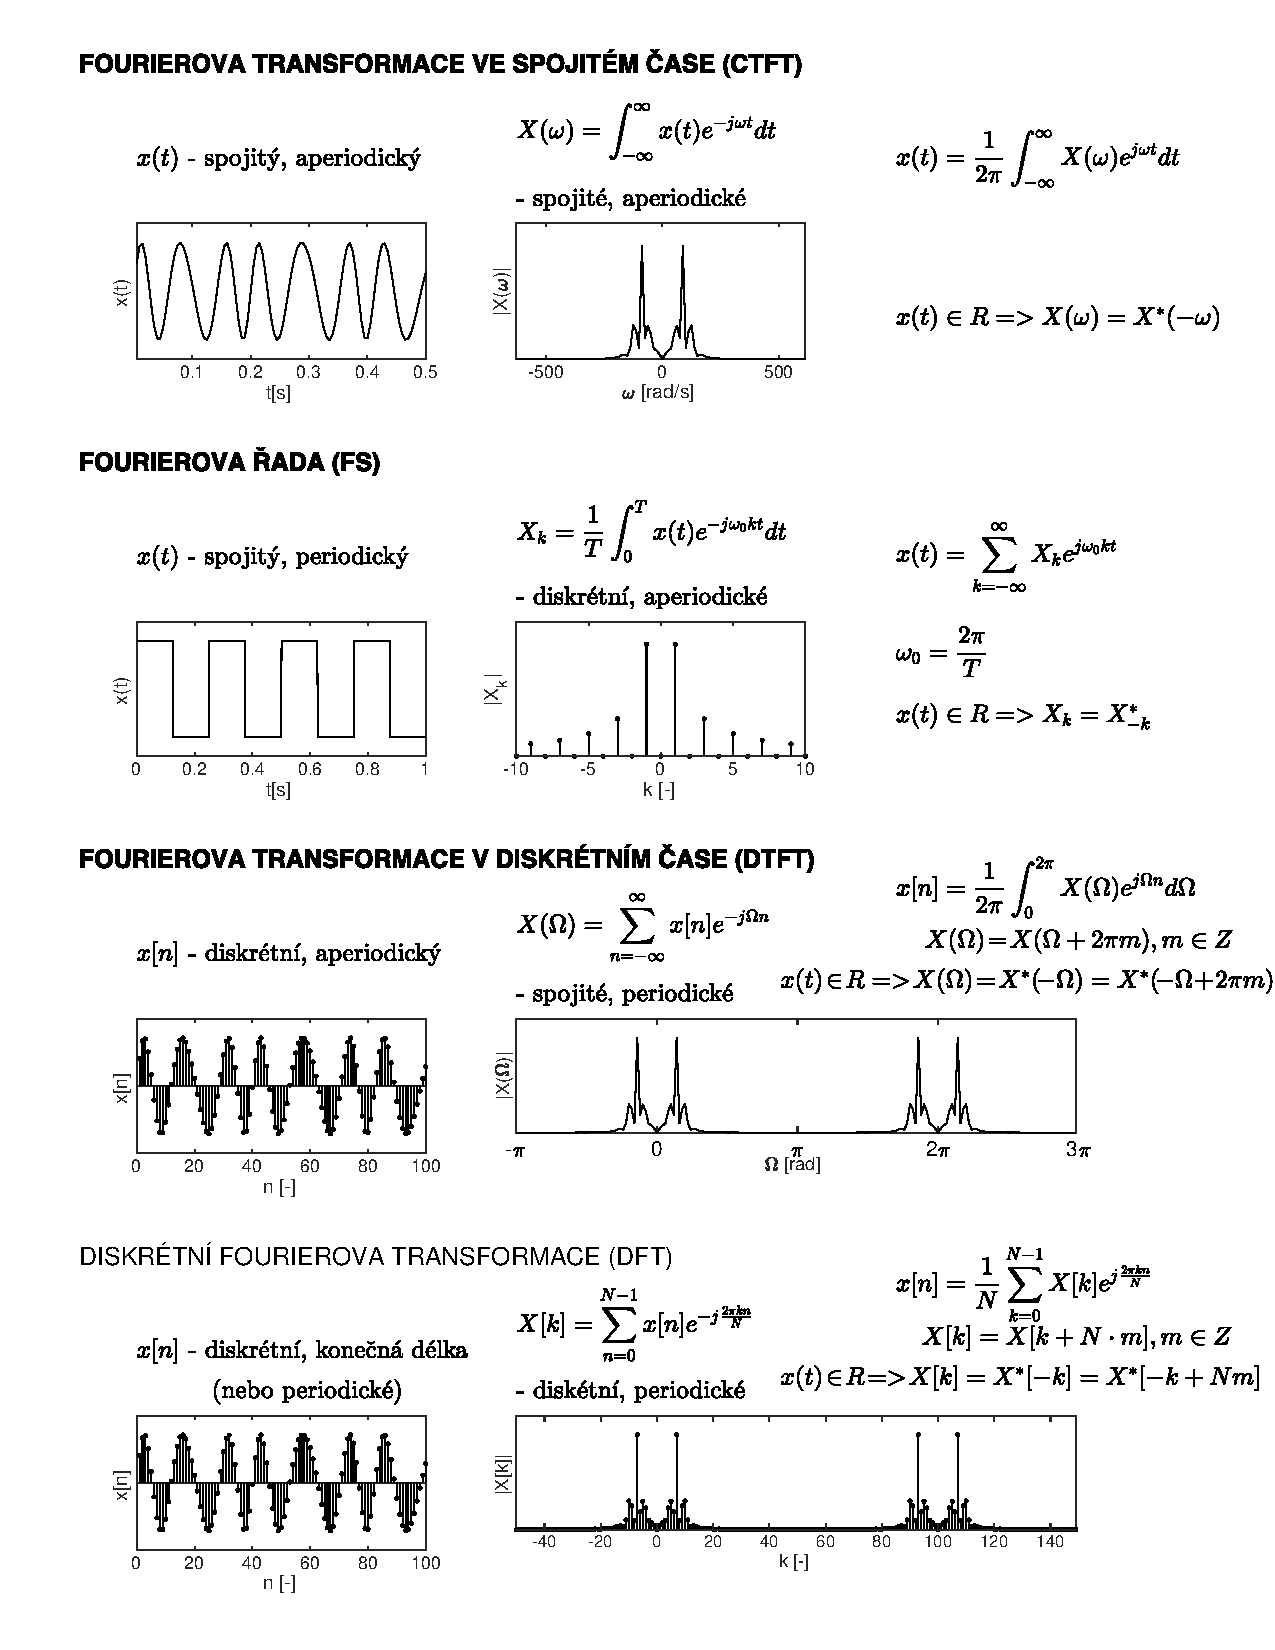
\includepdf{Fourierovy transformace CZ.pdf}  %[page={page number}]
	\subsection*{Fourierovy transformace}
		Fourierova transformace ve spojitém čase (CTFT)
			\[\mathcal{F}\{x(t)\} = X(\omega) 
			= \int_{-\infty}^{\infty} x(t)e^{-j\omega t} dt\]

		inverzní CTFT 
			\[x(t) = \frac{1}{2\pi} 
			\int_{-\infty}^{\infty} X(\omega)e^{j\omega t}d\omega\]

		Fourierova transformace v diskrétním čase (DTFT) 
		\[X(\Omega) = \sum_{n = - \infty}^{\infty} x[n]e^{-j\Omega n}\]

		inverzní (DTFT) 
		\[x[n] = \frac{1}{2 \pi} \int_{0}^{2 \pi} X(\Omega ) e^{j \Omega n} d\Omega\]


		Diskrétní Fourierova Transformace (DFT)
		\[X[k] = \sum_{s=0}^{N-1} x[n] e^{-j \frac{2\pi}{N}kn}\]

		Inverzní DFT
		\[x_p[n] = \frac{1}{N} \sum_{s=0}^{N-1} X[k] e^{j \frac{2\pi}{N}kn}\]


\section*{týden 4}
	\subsection*{Filtrace ve spektrální oblasti}
		$H(\omega), H(\Omega), H[k]$ - Frekvenční charakteristika (odezva), to je to jaký frekvence to propuští/nepropouští.
		Filtruje ve spektrální oblasti, to znamená, že nahrajeme zvuk mikrofonem,
		ten pomocí fourierovy transofrmace přeneseme do spektrální oblasti a 
		tady ho pronásobíme frekvenční charakteristikou, zpětnou fourierovou transformací
		to přeneseme zpět do časové oblasti a tam máme přefiltrovanej signál.\\\\
		Čtyři druhy frekvenčních charakteristik
		\begin{itemize}
			\item Dolní propust
			\item Horní propust
			\item Pásmová zádrž
			\item Pásmová propust
		\end{itemize}


		Nevýhody filtrování ve frekvenční oblasti: Musíme uložit celý signál, není v reálném čase

		\begin{center}
			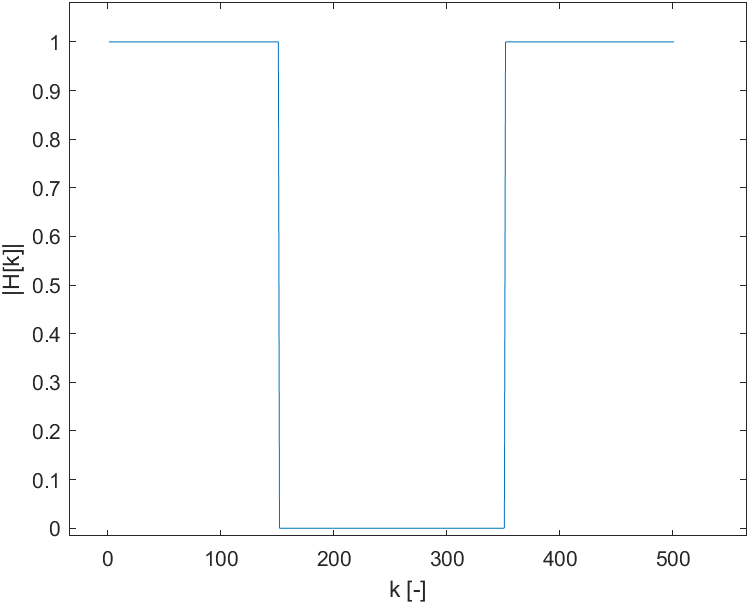
\includegraphics{untitled1.png}
		\end{center}
		
	\subsection*{Filtrace v časové oblasti}
		\subparagraph*{Lineární konvoluce}
		\[x[n] \ast y[n] = \sum_{m=-\infty}^{\infty}x[n-m]y[m]
		= \sum_{m = -\infty}^{\infty}x[m]y[n-m]\]
		\[x(t) \ast y(t) = \int_{-\infty}^{\infty} x(t-\tau)y(\tau)d\tau
		= \int_{-\infty}^{\infty}x(\tau) y(t-\tau)d\tau\]

	\subsection*{FIR filtry}
	\begin{center}
		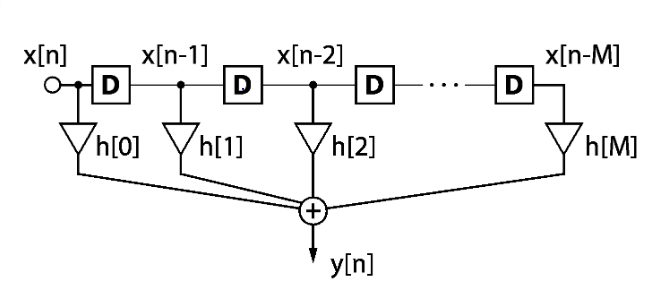
\includegraphics{FIR.png}
	\end{center}
		
	
		
\section*{týden 5}
$\delta[n] * h[n] =h[n]$ - impulsní odezva\\
$1\cdot H(\Omega)=H(\Omega)$ - frekvenční charakteristika

	\subsection*{IIR filtry}
	\begin{center}
		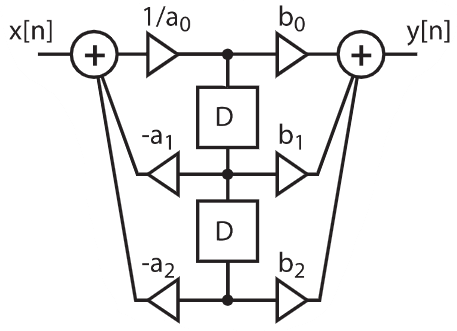
\includegraphics{IIR.png}
	\end{center}
	Nízký řád filtru - výpočetní náročnost je nízká\\
	Impulsní odezva nekonečná\\
	Data "obíhají" do nekonečna\\
	$a_0y[n]+a_1y[n-1]+a_2y[n-2]=b_0x[n]+b_1x[n-1]+b_2x[n-2] $ Difernční rovnice
\section*{týden 6}
	\subsection*{Popis spojitých LTI systémů}
		diskrétní systémy - difernční rovnice\\
		spojité systémy - diferenciální rovnice\\
		\subsection*{Homogenní systémy}
			Homogenní systémy jsou bez vstupu $(x(t)=0)$\\
			$a_2y''(t)+a_1y'(t)+a_0y(t)=0$ prostě se řeší diferenciální rovnice
			typické odezvy: podle toho kde vyjdou kořeny diff. rovnice.

			\begin{center}
				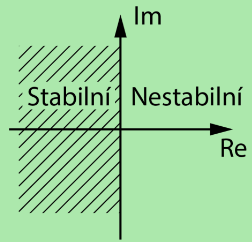
\includegraphics{stabilita.png}
			\end{center}



	\subparagraph*{Relativní tlumení $\zeta$ a vlastní úhlová frekvence $\omega_0$} 
			$y''(t)+2\zeta\omega_0 y'(t)+\omega_0^2$\\
			$\zeta > 1$ - nadkriticky tlumený systém\\
			$0 < \zeta < 1$ - podkriticky tlumený systém\\
			$\zeta = 0$ - netlumený systém\\
			$\zeta = 1$ - kriticky tlumený systém\\
			$\zeta < 0$ - nestabilní systém\\
			
		(vlastní úhlová frekvence je frekvence netlumených kmitů)

	\subsection*{Nehomogenní systémy}
		$a_2y''(t)+a_1y'(t)+a_0y(t)=b_0x(t)+b_1x'(t)+b_2x''(t)$\\
		Přepsat do frekvenční charakteristiky
		\[H(j\omega)=\frac{b_0+b_1j\omega+b_2(j\omega)^2}{a_0+a_1j\omega+a_2(j\omega)^2}\]
		\[Y(\omega)=X(\omega)H(j\omega)\overset{\mathcal{F}^{-1}}{\rightarrow}y(t)=x(t)*h(t)\]
		Bodeho charakteristika

\section*{týden 7}
	\subsection*{Laplaceova transformace}
		\[\mathcal{L}\{x(t)\}=\int_{0}^{\infty}x(t)e^{-st}dt\]
		Obrazy základních funkcí
		{\Large
		\begin{center}
			\begin{tabular}{| m{15em} | m{5em}|}\hline
				$\delta(t)$&$1$\\\hline
				${\bf 1}(t)$&$\frac{1}{s}$\\\hline
				$e^{at}{\bf 1}(t)$&$\frac{1}{s-a}$\\\hline
				$\cos(\omega t){\bf 1}(t)$&$\frac{s}{s^2+\omega^2}$\\\hline
				$\sin(\omega t){\bf 1}(t)$&$\frac{\omega}{s^2+\omega^2}$\\\hline
			\end{tabular}
		\end{center}
		}
		
\section*{týden 8}
	Statický systém - nemá póly v nule\\
	Astatický systém - má póly v nule
	\subsection*{Z-transformace}
	\[\mathcal{Z}\{x[n]\}=\sum_{n=0}^{\infty}x[n]z^{-n}=X(z)\]






\section*{týden 9}
	\subsubsection*{Z-transformace}
		Definice
		\[\mathcal{Z}\{x[n]\}=\sum_{n=0}^{\infty}x[n]z^{-n}\]

	{\Large
	\begin{center}
		\begin{tabular}{| m{15em} | m{5em}|}\hline
			$\delta(t)$&$1$\\\hline
			${\bf 1}(t)$&$\frac{z}{z-1}$\\\hline
			$a^n{\bf 1}(t)$&$\frac{z}{z-a}$\\\hline
		\end{tabular}
	\end{center}
	}
\section*{týden 10}
	\subsection*{Popis LTI systémů}
		Prostě náčrty systémů
\section*{týden 11}
	\subsection*{Linearizace}
		Hledání pracovního bodu.......
\section*{týden 12}
	\subsection*{Diskretizace}
	$(T_s)$ je vzorkovací perioda
	\begin{itemize}
		\item Dopředná diference
			\[s=\frac{z-1}{T_s}\]
		\item Zpětná diference
			\[s=\frac{1-z^{-1}}{T_s}\]
		\item Bilineární transformace
			\[s=\frac{2}{T_s}\frac{1-z^{-1}}{1+z^{-1}}\]
		\item Impulsní invariance\\
			Provede se zpětný laplace, všechny $t$ se nahradí $\frac{n}{T_s}$,
			a to se z-transformuje
		\item Metoda mapování nul a pólů\\
			Najdou se nuly a póly, ty se nahraděj pólama z prostoru z
			(pól je $\omega$ do z jako $e^{\frac{\omega}{T_s}}$)
	\end{itemize}
\section*{týden 13}
	\subsection*{Modulace}
		Máme náhravku třeba lidský řeči (20Hz - 20kHz) a potřebujeme jí poslat, kdybychom
		chtěli poslat přímo frekvenci kterou posíláme, tak nebudeme mít dost velkou anténu, 
		musíme to posunout do vyšších frekvencí

		\subparagraph*{Amplitudová modulace}
			Nosnému signálu měníme amplitudu podle hodnot modulačního signálu.\\
			$y(t) = (1+m\cdot x_m(t))\cdot\cos(\omega_c t)$\\
			Kosinus představuje  nosný signál, $\omega_c$ je frekvence nosného signálu
			to $m \cdot x_m(t)$ je modulační signál

			Demodulace - usměrnění signálu a low pass filtr

		
		\subparagraph*{QAM - Kvadrální amplitudová modulace}

		\subparagraph*{Frekvenční modulace}

		\subparagraph*{Fázová modulace}

		\subparagraph*{Hilbertova Transformace}
			\[x_H(t)=\int_{-\infty}^{\infty}\frac{1}{t-\tau}x(\tau)ft\]

\section*{týden 14}		
Odvození vzorců
\[\mathcal{Z}\{\delta[n]\}=\sum_{n=0}^{\infty}\delta[n]z^{-n}=z^0=1\]
impulsní odezva se zjštuje, tak že najdeme Z/L transformaci
a přechodovou odezvu (odezva na jednotkový skok) najdeme tak,
že zase najdem Z/L transformaci ale pronásonbenou 
zpětnou Z/L transformací jednotkovýho skoku
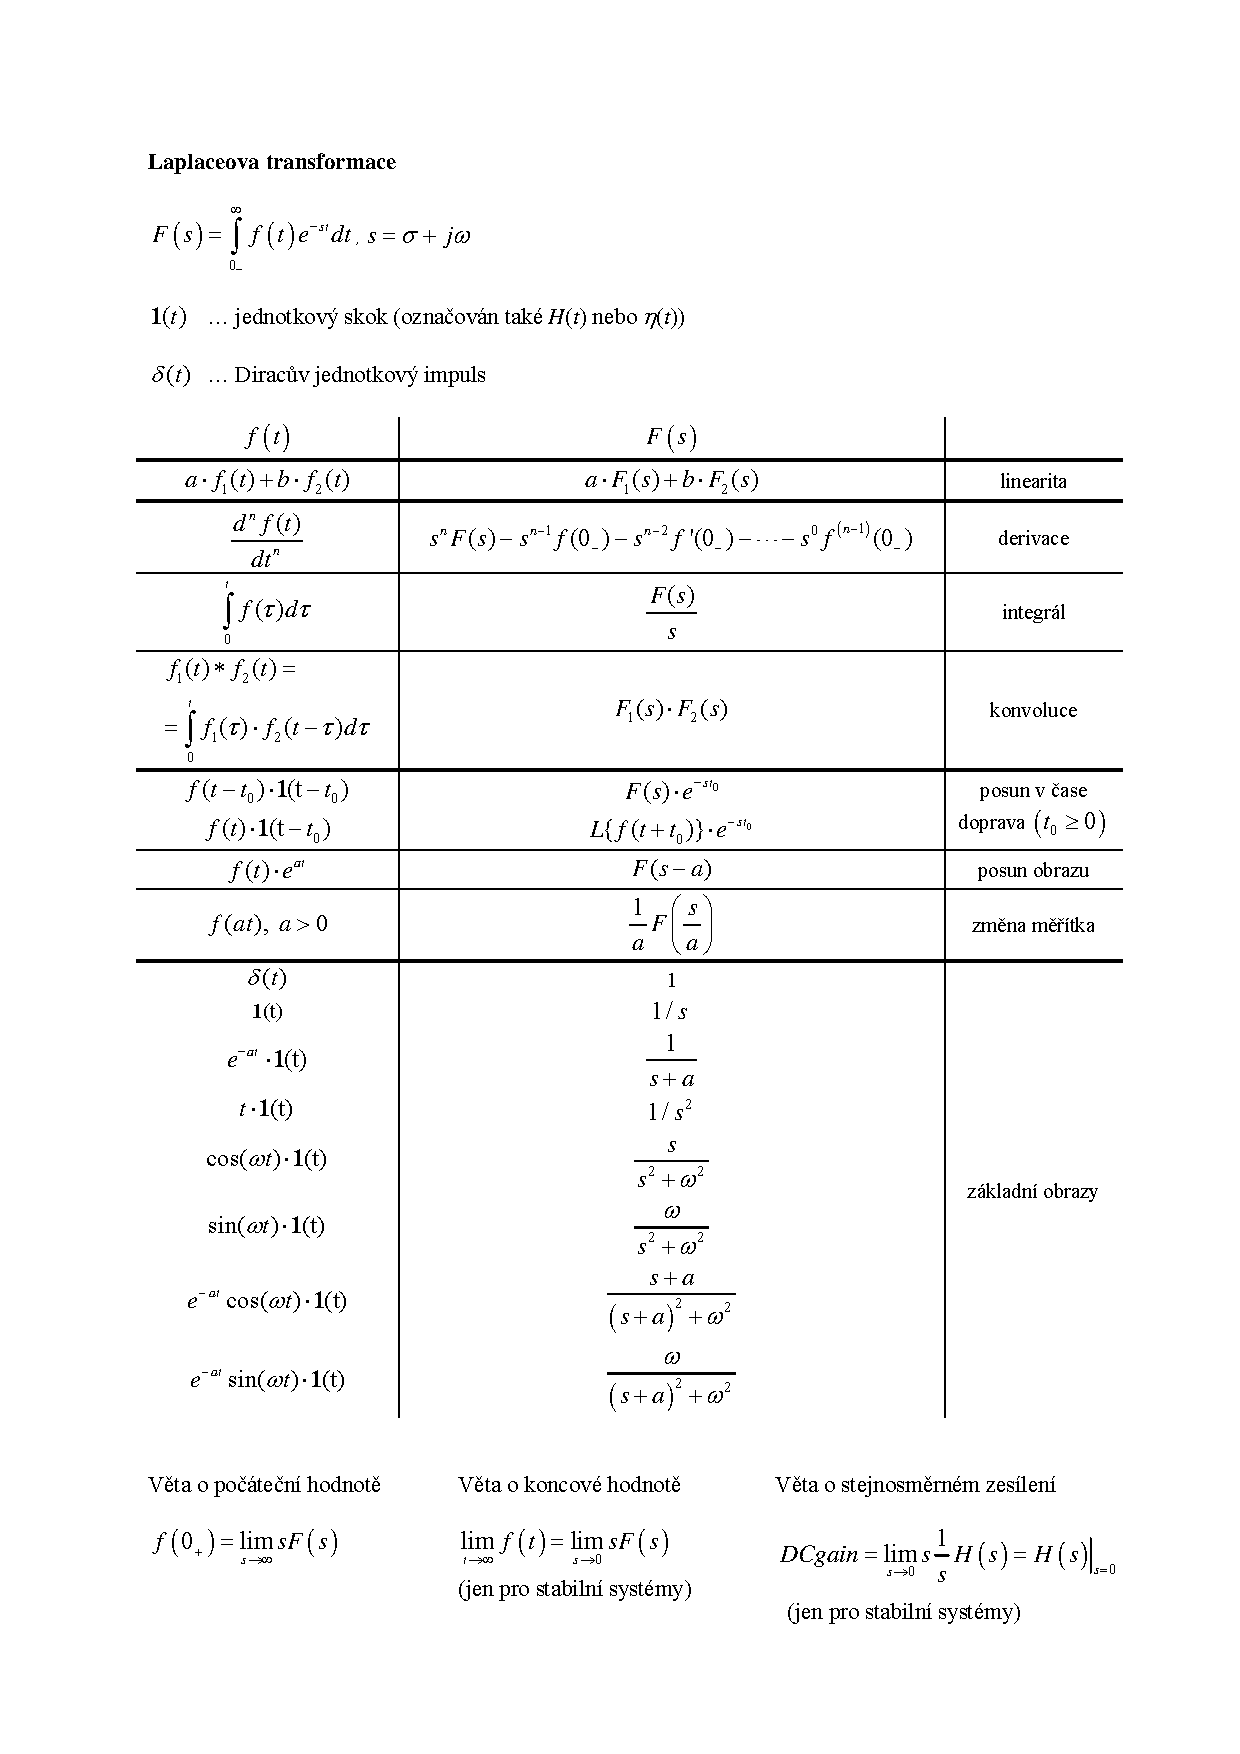
\includepdf{slovnik_lt.pdf}
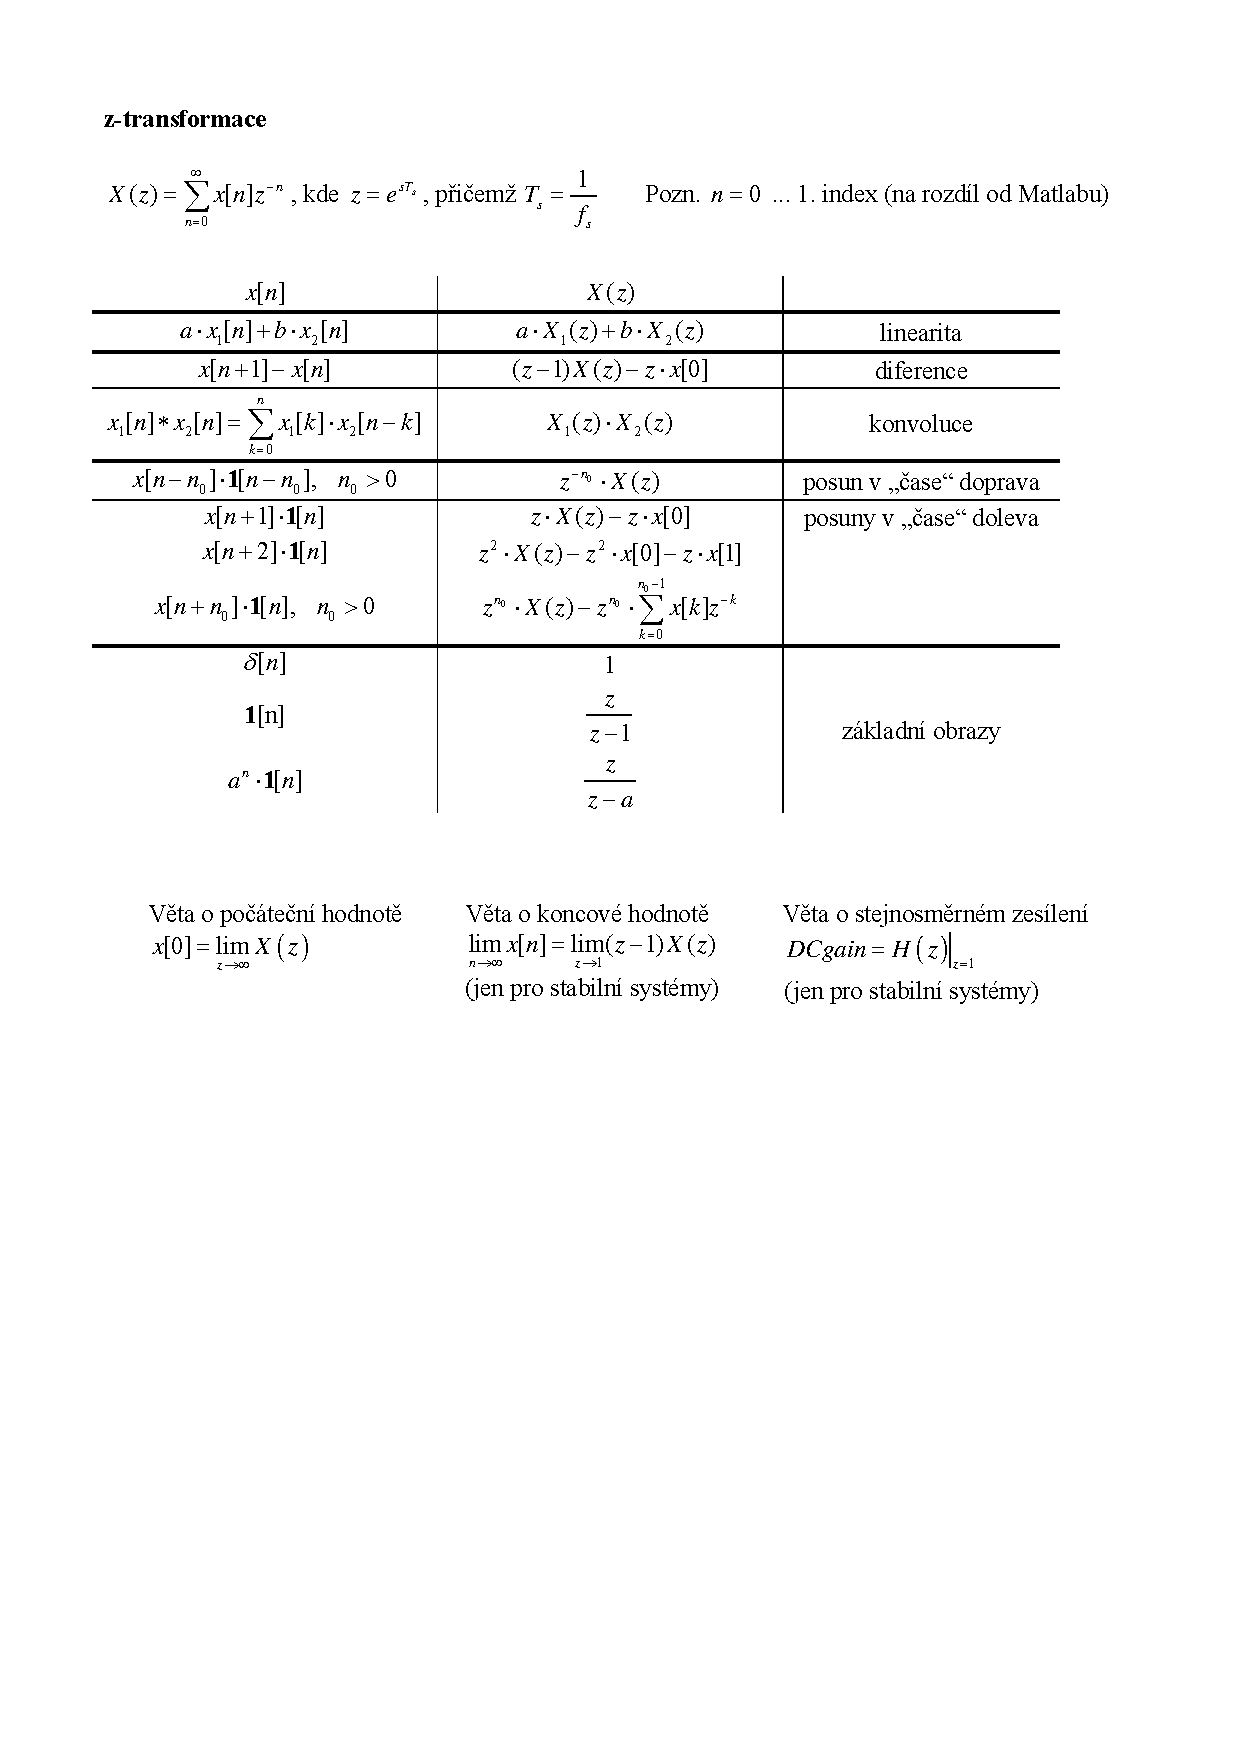
\includepdf{slovnik_zt.pdf}
	frekvenční charakteristika je to jaký frekvence potlačujeme a jaký necháváme/zesilujeme\\
	lineární konvoluce je filtrování v časový oblasti
	Časová oblsat - to co slyší mirofon - signál
	spektrální oblsat - to co slyší ucho - spektrum - dostaneme fourierovou transformací
	
	Nevýhoda filtrování ve spektrální oblasti
	\begin{itemize}
		\item Musíme uložit celý signál
		\item Není v reálném čase
	\end{itemize}
	\begin{center}
		\begin{tabular}{|c|c|c|}
			\hline
			$H(\Omega), H(\omega), H[k]$ & Frekvenční charakteristika & To jaký frekvence jsou potlačený/ponechaný/zesílený\\
			$Y(\Omega)$&&To co zbude po vynásobení signálu s $H(\Omega)$\\
			$h[n]$&impulsní odezva& $H(\omega)=\mathcal{F}\{h(t)\}, H(\Omega)= \mathcal{F}\{h[n]\}$\\
			&&\\
			&&\\
			&&\\
			&&\\
			\hline
		\end{tabular}
	\end{center}
	

	LTI systém popsaný nějakou diferenciální rovnicí
	\[y''(t)+5'(t)+6y(t)=x'(t)+6x(t)\]
	\\
	Najít póly a nuly - přepsat si rovnici
	\[0=\frac{\lambda+6}{\lambda^2+5\lambda+6}=\frac{\lambda+6}{(\lambda+2)(\lambda+3)}\]
	Nuly jsou tamm kde funkce nabývá nule, póly, tam kde nabývá nekonečna - prostě singularity 
	\\
	\\
	impulsní charakteristika - inverzní laplace
	\\
	\\
	přechodová charakteristika - (odezva na jednotkový skok) - pronásoobené laplasovanym
	jednotkovym skokem $(\frac{1}{s})$ a inverzní lapace
	\\
	\\
	hodnoty přechodové charakteristiky - jenom se dosadí do přechodové charakteristiky
	\\
	\\
	Vypočítat výstup systému na nějakej vstup - je to jako přechodová charakteristika ale
	na vstupu není jednotkovej skok ale něco jinýho
\end{document}